\documentclass[a4paper]{article}
\usepackage{svn-multi}
% Version control information:
\svnidlong
{$HeadURL: https://practicas-derive.googlecode.com/svn/trunk/espacios_vectoriales.tex $}
{$LastChangedDate: 2008-11-13 12:37:02 +0100 (jue, 13 nov 2008) $}
{$LastChangedRevision: 3 $}
{$LastChangedBy: asalber $}
\svnid{$Id: espacios_vectoriales.tex 3 2008-11-13 11:37:02Z asalber $}
\pdfinfo{/CreationDate (D:\svnpdfdate)}
\svnRegisterAuthor{alf}{Alfredo Sánchez Alberca}

\usepackage[spanish]{babel}
\usepackage[utf8x]{inputenc}
\usepackage{amsmath}
\usepackage{macros}
\usepackage[dvips]{graphicx}
\usepackage{enumitem}
\usepackage{subfigure}
\usepackage[small,bf]{caption2}
\usepackage[top=3cm, bottom=3cm, left=2.54cm, right=2.54cm]{geometry}
\usepackage{fancyhdr}
\pagestyle{fancy}

\lhead{\textsc{Universidad San Pablo CEU}} \rhead{\textsl{\textsf{Departamento de Métodos Cuantitativos}}}
\renewcommand{\headrulewidth}{0pt}
\renewcommand{\floatpagefraction}{.8}
\renewcommand{\textfraction}{.1}
\setcaptionwidth{\textwidth} \addtolength{\captionwidth}{-40pt}
\captionstyle{indent} \setlength\captionindent{\parindent}

\makeatletter
\let\savees@listquot\es@listquot
\def\es@listquot{\protect\savees@listquot}
\makeatletter

\begin{document}
\sloppy \practica{Práctica de Álgebra con Derive}{Espacios Vectoriales}

\bigskip
\section*{Fundamentos Teóricos}
Los espacios vectoriales son la esencia del álgebra lineal. En muchos problemas de física, ingeniería o estadístcia se trabaja sobre conjuntos conocidos como $R^2$, $R^3$ o $R^n$ en general, que son espacios vectoriales. Conocer la estructura de este tipo de conjuntos y las propiedades que de ella se derivan resulta imprescindible en la resolución de estos problemas. En esta práctica introducimos el concepto de espacio vectorial y también el concepto de dependencia lineal y se muestra cómo trabajar con estos conceptos en Derive. 

\subsection*{Espacio vectorial}
Sea $K$ un cuerpo cuyos elementos llamaremos \emph{escalares}, y $V$ un
conjunto no vacío cuyos elementos llamaremos \emph{vectores}, en el que se ha
definido una operación interna $+$ llamada suma de vectores ($\forall\,
\mathbf{u},\mathbf{v}\in V,\ \mathbf{u}+\mathbf{v}\in V$) y una operación
externa $\cdot$ llamada producto por escalar ($\forall\, a\in K, \mathbf{v}\in
V,\ a\cdot \mathbf{v}\in V$). Diremos que $V$ tiene estructura de \emph{espacio
vectorial} sobre $K$, si se cumplen las siguientes propiedades.
\begin{enumerate}
\item Para la suma, $(V,+)$ es un grupo abeliano, es decir, se cumple:
\begin{enumerate}
\item Propiedad Asociativa: $\forall\, \mathbf{u},\mathbf{v},\mathbf{w}\in V,\
 (\mathbf{u}+\mathbf{v})+\mathbf{w}=\mathbf{u}+(\mathbf{v}+\mathbf{w})$.
\item Propiedad Conmutativa: $\forall\, \mathbf{u},\mathbf{v}\in V,\
\mathbf{u}+\mathbf{v}=\mathbf{v}+\mathbf{u}$.
\item Elemento Neutro: Existe un vector $\mathbf{0}\in V$ tal que $\forall\, \mathbf{v}\in V,\
\mathbf{0}+\mathbf{v}=\mathbf{v}$.
\item Elemento Opuesto: $\forall\, \mathbf{v}\in V$, existe un vector $\mathbf{-v}\in V$, tal que
$\mathbf{v}+(\mathbf{-v})=\mathbf{0}$.
\end{enumerate}
\item Para el producto por escalar se cumple:
\begin{enumerate}
\item Propiedad Distributiva respecto a la suma de escalares: $\forall\,
a,b\in K,\mathbf{v}\in V,\ (a+b)\cdot \mathbf{v}=a\cdot \mathbf{v}+b\cdot
\mathbf{v}$.
\item Propiedad Distributiva respecto a la suma de vectores:$\forall\,
a\in K,\mathbf{u},\mathbf{v}\in V,\ a\cdot (\mathbf{u}+\mathbf{v})=a\cdot
\mathbf{u}+a\cdot \mathbf{v}$.
\item Propiedad Seudoasociativa: $\forall\,
a,b\in K,\mathbf{v}\in V,\ (a\cdot b)\cdot \mathbf{v}=a\cdot (b\cdot
\mathbf{v})$.
\item Elemento Unidad: Existe un escalar 1, tal que $\forall\, \mathbf{v}\in V,\ 1\cdot
\mathbf{v}=\mathbf{v}$.
\end{enumerate}
\end{enumerate}

\begin{ejemplo}
El conjunto de pares ordenados $\mathbb{R}^2=\{(x,y):x.y\in \mathbb{R}\}$ con
la operación suma definida del siguiente modo
\[
(x_1,y_1)+(x_2,y_2)=(x_1+x_2,y_1+y_2),
\]
y la operación producto por escalar definida de la forma
\[
a\cdot(x_1,y_1)=(ax_1,ay_1),
\]
tiene estructura de espacio vectorial sobre $\mathbb{R}$.

Desde el punto de vista geométrico, los vectores de este espacio vectorial
pueden representarse como segmentos orientados en el plano cartesiano
$\mathbb{R}^2$, con origen en el origen de coordenadas, tal y como se muestra en la figura~\ref{g:coordenadascartesianas}. 

\begin{figure}[h!]
\begin{center}
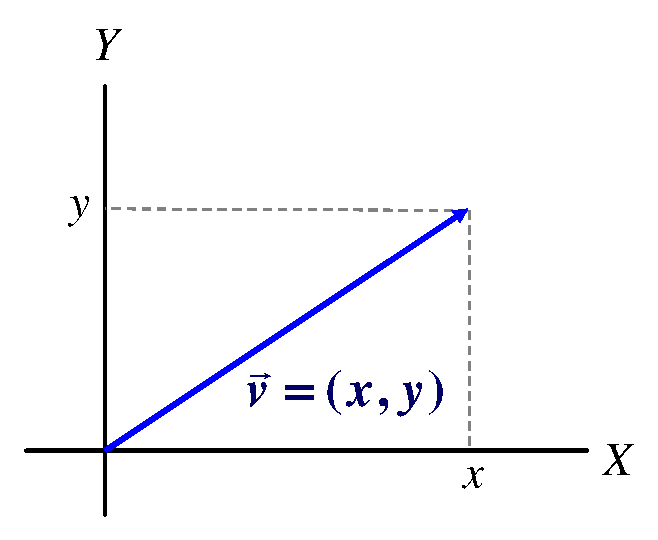
\includegraphics[scale=0.5]{coordenadascartesianas}
\caption{Vectores del espacio vectorial $\mathbb{R}^2$. Cada vector está determinado por un par de coordenadas $(x,y)$.}
\label{g:coordenadascartesianas}
\end{center}
\end{figure}

Otro ejemplo de espacio vectorial sobre $\mathbb{R}$ es el conjunto
$\mathcal{P}(x)$ de los polinomios en la variable $x$ con coeficientes reales
con las operaciones habituales de suma de polinomios y producto por un valor
real, tiene estructura de espacio vectorial sobre. Sin embargo, el conjunto
$\mathcal{P}^n(x)$ de los polinomios de grado $n$ en la variable $x$ con
coeficientes reales y las mismas operaciones que antes, no tendría estructura
de espacio vectorial, ya que, en general, no se cumple que la suma de
polinomios de grado $n$ sea un polinomio de grado $n$.
\end{ejemplo}

\subsection*{Subespacio vectorial}
Sea $V$ un espacio vectorial sobre $K$ y $W$ un subconjunto no vacío de $V$. Diremos que $W$ es un \emph{subespacio vectorial} de $V$ sobre $K$, si $W$, con las operaciones de $V$, es a su vez espacio vectorial sobre $K$.
En general, para que $W\subseteq V$ sea subespacio vectorial de $V$, basta con que se verifique:
\begin{enumerate}
\item $\forall\, \mathbf{u},\mathbf{v}\in W,\  \mathbf{u}+\mathbf{v}\in W$.
\item $\forall\, a\in K,\ \mathbf{u}\in W,\ a\cdot \mathbf{u}\in W$.
\end{enumerate}
o lo que es lo mismo $\forall\, a,b\in K,\ \mathbf{u},\mathbf{v}\in W,\  a\cdot \mathbf{u}+b\cdot \mathbf{v}\in W$.

Cualquier espacio vectorial $V$ tiene dos subespacios vectoriales triviales: el propio espacio $V$ y el subconjunto formado por el elemento neutro $W={\mathbf{0}}$.

\subsection*{Combinación lineal}
Diremos que un vector $\mathbf{v}\in V$ es \emph{combinación lineal} de los vectores $\mathbf{v_1},\ldots,\mathbf{v_n}$ si existen escalares $a_1,...,a_n\in K$, tales que
\[\mathbf{v }= a_1\mathbf{v_1}+\cdots+ a_n\mathbf{v_n}=\sum_{i=1}^n{a_i\mathbf{v_i}}.\]

\begin{ejemplo}
Si consideramos los vectores $\mathbf{v_1}=(1,1,1)$, $\mathbf{v_2}=(1,1,0)$ y $\mathbf{v_3}=(0,0,1)$ de $\mathbb{R}^3$, entonces el vector $\mathbf{v}=(3,3,1)$ es combinación lineal de $\mathbf{v_1}$, $\mathbf{v_2}$ y $\mathbf{v_3}$ ya que puede escribirse como $\mathbf{v}=2 \mathbf{v_1}+ \mathbf{v_2}- \mathbf{v_3}$.
\end{ejemplo}

El conjunto de todos los vectores que pueden escribirse como combinación lineal de $\mathbf{v_1},\ldots,\mathbf{v_n}\in V$, que se denotará por $L(\mathbf{v_1},\ldots,\mathbf{v_n})$, se llama \emph{clausura lineal} de $\mathbf{v_1},\ldots,\mathbf{v_n}$ y es un subespacio vectorial de $V$.

\subsection*{Sistema de generadores de un espacio vectorial}
Sea $W$ un subespacio vectorial de $V$. Diremos que un conjunto de vectores $\mathbf{v_1},\ldots,\mathbf{v_n}\in W$ es un \emph{sistema de generadores} de $W$, si  $W=L(\mathbf{v_1},\ldots,\mathbf{v_n})$, es decir, si todo vector de $W$ se puede expresar como combinación lineal de $\mathbf{v_1},\ldots,\mathbf{v_n}$,
\[ \forall\, \mathbf{v}\in W \exists a_1,\ldots,a_n\in K,,  \mathbf{v} = a_1\mathbf{v_1}+\cdots+ a_n\mathbf{v_n}.\]

\subsection*{Dependencia lineal}
Diremos los vectores $\mathbf{v_1},\ldots,\mathbf{v_n}\in V$ $(n>1)$ son \emph{linealmente dependientes}, si al menos uno de estos vectores puede escribirse como combinación lineal de los restantes. De lo contrario, diremos que son \emph{linealmente independientes}.

Una forma de ver si un conjunto de vectores $\mathbf{v_1},\ldots,\mathbf{v_n}\in V$ son linealmente independientes es ver si existen escalares $a_1,\ldots,a_n\in K$ no nulos, tales que
\[a_1\mathbf{v_1}+\cdots+ a_n\mathbf{v_n}=0.\]
Por el contrario, si los únicos escalares que cumplen la ecuación son $a_1=a_2=\cdots=a_n=0$, entonces los vectores serán linealmente independientes.

Al número máximo de vectores linealmente independientes de un conjunto de vectores se le llama \emph{rango}.

\subsection*{Base y dimensión de un espacio vectorial}
Diremos que un subconjunto de vectores $B=\{\mathbf{v_1},\ldots,\mathbf{v_n}\}\subset V$ es una \emph{base} del espacio vectorial $V$, si y sólo si se cumplen las dos condiciones siguientes:
\begin{enumerate}
\item $B$ es un sistema de generadores de $V$.
\item Los vectores de $B$ son linealmente independientes.
\end{enumerate}

Cualquier espacio vectorial $V\neq\{\mathbf{0}\}$ tiene una base, y además, no es única.
Se puede comprobar además, que todas las bases de un espacio vectorial  engendrado por un número finito de elementos tienen el mismo número de elementos, y en consecuencia, llamaremos \emph{dimensión} de un espacio vectorial $V$, al número de elementos de cualquiera de sus bases, y se nota $\textrm{Dim}(V)$.

\subsubsection*{Coordenadas con respecto a una base}
Una base de un espacio vectorial $V$, al ser un sistema de generadores de $V$, permite escribir cualquier vector $\mathbf{v}$ como combinación lineal de los elementos de $B$. Además, al ser los vectores de $B$ linealmente independientes, la forma de expresar $v$ como combinación lineal de los elementos de $B$ es única.

Así pues, dada una base $B=\{\mathbf{v_1},\ldots,\mathbf{v_n}\}$ de un espacio vectorial $V$ se dice que $a_1,\ldots,a_n\in K$ son las \emph{coordenadas} de $\mathbf{v}\in V$ con respecto a la base $B$ si y sólo si
\[\mathbf{v }= a_1\mathbf{v_1}+\cdots+ a_n\mathbf{v_n}.\]

\begin{figure}[h!]
\begin{center}
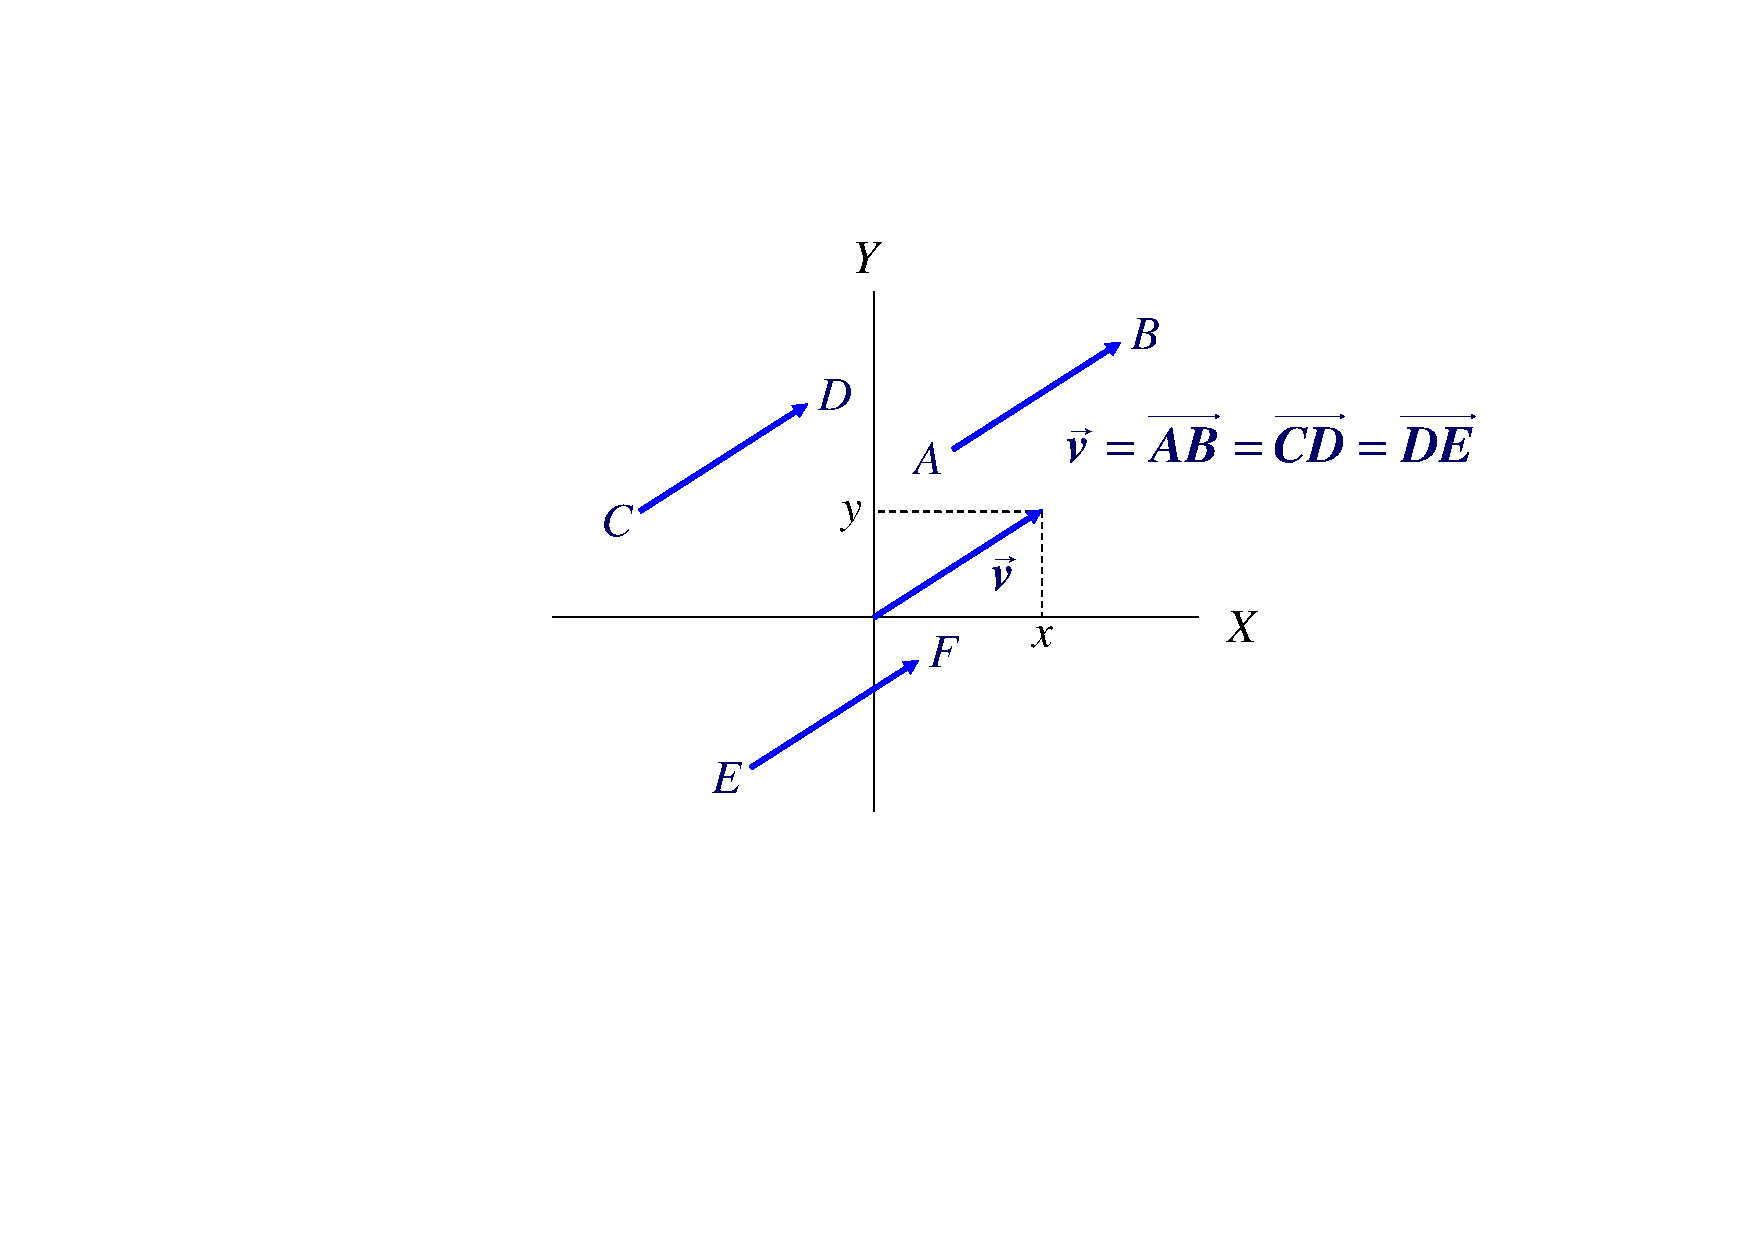
\includegraphics[scale=0.5]{coordenadas}
\caption{Coordenadas de un vector en $\mathbb{R}^2$ con respecto a distintas bases.}
\label{g:coordenadas}
\end{center}
\end{figure}

En un espacio vectorial $K^n$, se define la \emph{base canónica} como $B_c=\{e_1,\ldots,e_n\}$, siendo $e_i=(e_{i1},\ldots,e_{in})$, donde 
\[e_{ij}=
\left\{%
\begin{array}{ll}
    1, & \hbox{si $i=j$;} \\
    0, & \hbox{si $i\neq j$.} \\
\end{array}%
\right.    
\]

\begin{ejemplo}
La base canónica de $\mathbf{R^3}$ es $B_c=\{(1,0,0), (0,1,0), (0,0,1)\}$.
\end{ejemplo}

La base canónica tiene muy buenas propiedades ya que está formada por vectores ortonormales y además las coordenadas de cualquier vector con respecto a $B_c$ coinciden con sus componentes en el sistema cartesiano.

\section*{Ejercicios Prácticos}
\begin{enumerate}[leftmargin=*]
\item Dados los vectores $\mathbf{u}=(1,-1,0)$, $\mathbf{v}=(2,3,-1)$ y $\mathbf{w}=(1,-6,-1)$ de $\mathbb{R}^3$, hallar los escalares $a,b\in \mathbb{R}$ que permitan expresar el vector $\mathbf{w}$ como combinación lineal de $\mathbf{u}$ y $\mathbf{v}$.

\item Averiguar si los vectores $v_1=(0,-1,2,0)$, $v_2=(1,3,0,-1)$, $v_3=(1,-8,8,1)$ y $v_4=(1,-1,1,0)$ son linealmente independientes. Si no es así, ¿cuál es el mayor número de vectores linealmente independientes de este conjunto?

\item Sea $S=\{(1,1,2,0),(2,-1,0,1),(5,-1,2,2),(3,0,2,1)\}\subset \mathbb{R}^4$ y sea $H$ el subespacio vectorial generado por $S$. Se pide:
\begin{enumerate}
\item Calcular el rango de $S$.
\item Calcular una base de $H$.
\item Averiguar si los vectores $(2,11,16,-3)$ y $(1,3,2,5)$ pertenecen a $H$.
\end{enumerate}

\item Determinar una base del subespacio de $\mathbb{R}^4$ engendrado por $\{(1,2,3,1),(2,3,2,3), (0,1,4,-1),$ $(2,-3,1,1),(4,1,7,3)\}$.

\item Comprobar que el subconjunto de vectores $B=\{(-1,0,1),(1,1,0),(1,2,3)\}$ son una base de $\mathbb{R}^3$ y hallar las coordenadas del vector $\mathbf{v}=(3,-1,2)$ respecto de $B$.

\item La coordenadas de un vector $\mathbf{w}$ respecto de la base $B=\{\mathbf{u_1},\mathbf{u_2}\}$ son $(-1,4)$. Hallar las coordenadas de $\mathbf{w}$ respecto de la base $B'=\{\mathbf{v_1},\mathbf{v_2}\}$ sabiendo que $\mathbf{u_1}=\mathbf{v_1}-\mathbf{v_2}$ y $\mathbf{u_2}=2\mathbf{v_1}-3\mathbf{v_2}$.

\end{enumerate}

\section*{Problemas}
\begin{enumerate}[leftmargin=*]

\item  Determinar para qué valor de $a$ el subespacio engendrado por el
conjunto de vectores $S=\{(1,1,0)$, $(3,a,2)$, $(0,1,a)\}$ será
$\mathbb{R}^{3}$.

\item El conjunto $B=\{-x^2+1,-x^2+x,x^2-2x+2\}$ es una base del espacio vectorial de los polinomios en $x$ de grado menos o igual que 2 $\mathcal{P}_2$. Dar las coordenadas con respecto a esta base del polinomio $-6x^2+x+3$. 

\item  Estudiar si son linealmente independientes las matrices
\[
A=\left(
\begin{array}{rr}
3 & -1 \\ 2 & 1
\end{array}
\right) ,\quad B=\left(
\begin{array}{rr}
-2 & 3 \\ -1 & -2
\end{array}
\right)\quad \mbox{y}\quad C=\left(
\begin{array}{rr}
5 & 3 \\ 4 & -1
\end{array}
\right) .
\]


\item En cierta base $B=\{\mathbf{u_1},\mathbf{u_2},\mathbf{u_3},\mathbf{u_4}\}$ de $R^4$, un vector $w$ tiene coordenadas $(3,1,2,6)$. Hallar las coordenadas de $w$ en otra base $B'=\{\mathbf{v_1},\mathbf{v_2},\mathbf{v_3},\mathbf{v_4}\}$ cuyos vectores verifican
\[
\mathbf{v_1}=3\mathbf{u_1}+4\mathbf{u_3} \quad \mathbf{v_2}=\mathbf{u_2}-\mathbf{u_4} \quad \mathbf{v_3}=\mathbf{u_1}+\mathbf{u_2}+\mathbf{u_3} \quad \mathbf{v_4}=3\mathbf{u_4}.
\]
\end{enumerate}


  




\end{document}
